\chapter{Nadajnik ultradźwiękowy}
\section{Budowa i zasada działania}

Nadajnik zbudowany został w oparciu o \textit{Arduino Nano} \cite{bib:arduinoNano} do którego podłączono 
bezpośrednio cztery nadajniki ultradźwiękowe (rezonatory piezoelektryczne) typu 40ST-12 \cite{bib:40ST12}, schemat 
przedstawiony jest na rysunku \ref{fig:nadajnik_schemat}.

\rysunek{transmitter}{schemat nadajnika ultradźwiękowego}{\label{fig:nadajnik_schemat}}


Całość umieszczona została w ramie w kształcie litery \textbf{H} wykonanej z rurek PCV.
Rezonatory zostały dodatkowo odizolowane od ramy rzepami co ułatwia ich zdejmowanie jak i skutecznie
zapobiega przenoszeniu się drgań.

\rysunek{nadajnik_H}{szkic ramy nadajnika}{\label{fig:nadajnik_szkic}}


Płytka połączona jest z odbiornikiem 6m przewodem, którym przesyłane są sygnały sterujące jak i zasilanie.
Do sterowania wykorzystywane są 3 przewody, dwa z nich informują który z rezonatorów ma w danym momencie nadawać,
trzeci służy jako wyzwalacz.

Cała logika oprogramowania mieści się w obsłudze przerwania sprzętowego, które reaguje na zmianą stanu logicznego
na wyzwalaczu,
po uruchomieniu przerwania oprogramowanie wysyła sygnał na odpowiedni rezonator. 
Nadany sygnał jest tak dobrany by dało się go w łatwy sposób odróżnić i składa się w dwóch
części: część wzbudzająca 
Długość impulsów jest zgodna z częstotliwością rezonansową nadajników, dodatkowo jeden
impuls jest przesunięty względem drugiego o 180 stopni. Pierwszy z nich ma za zadanie wzbudzić rezonator, a drugi wytłumić, 
tak by nadany sygnał był jak najkrótszy. 
Rysunek \ref{fig:output_signal} przedstawia sygnał jakim wysterowany jest przetwornik piezoelektryczny. 

Odległość między nadajnikiem a odbiornikami wyznaczany jest przez odbiornik na podstawie
czasu jaki potrzebował sygnał dźwiękowy by pokonać daną odległość.

 \begin{figure}[h!]
    \centering
    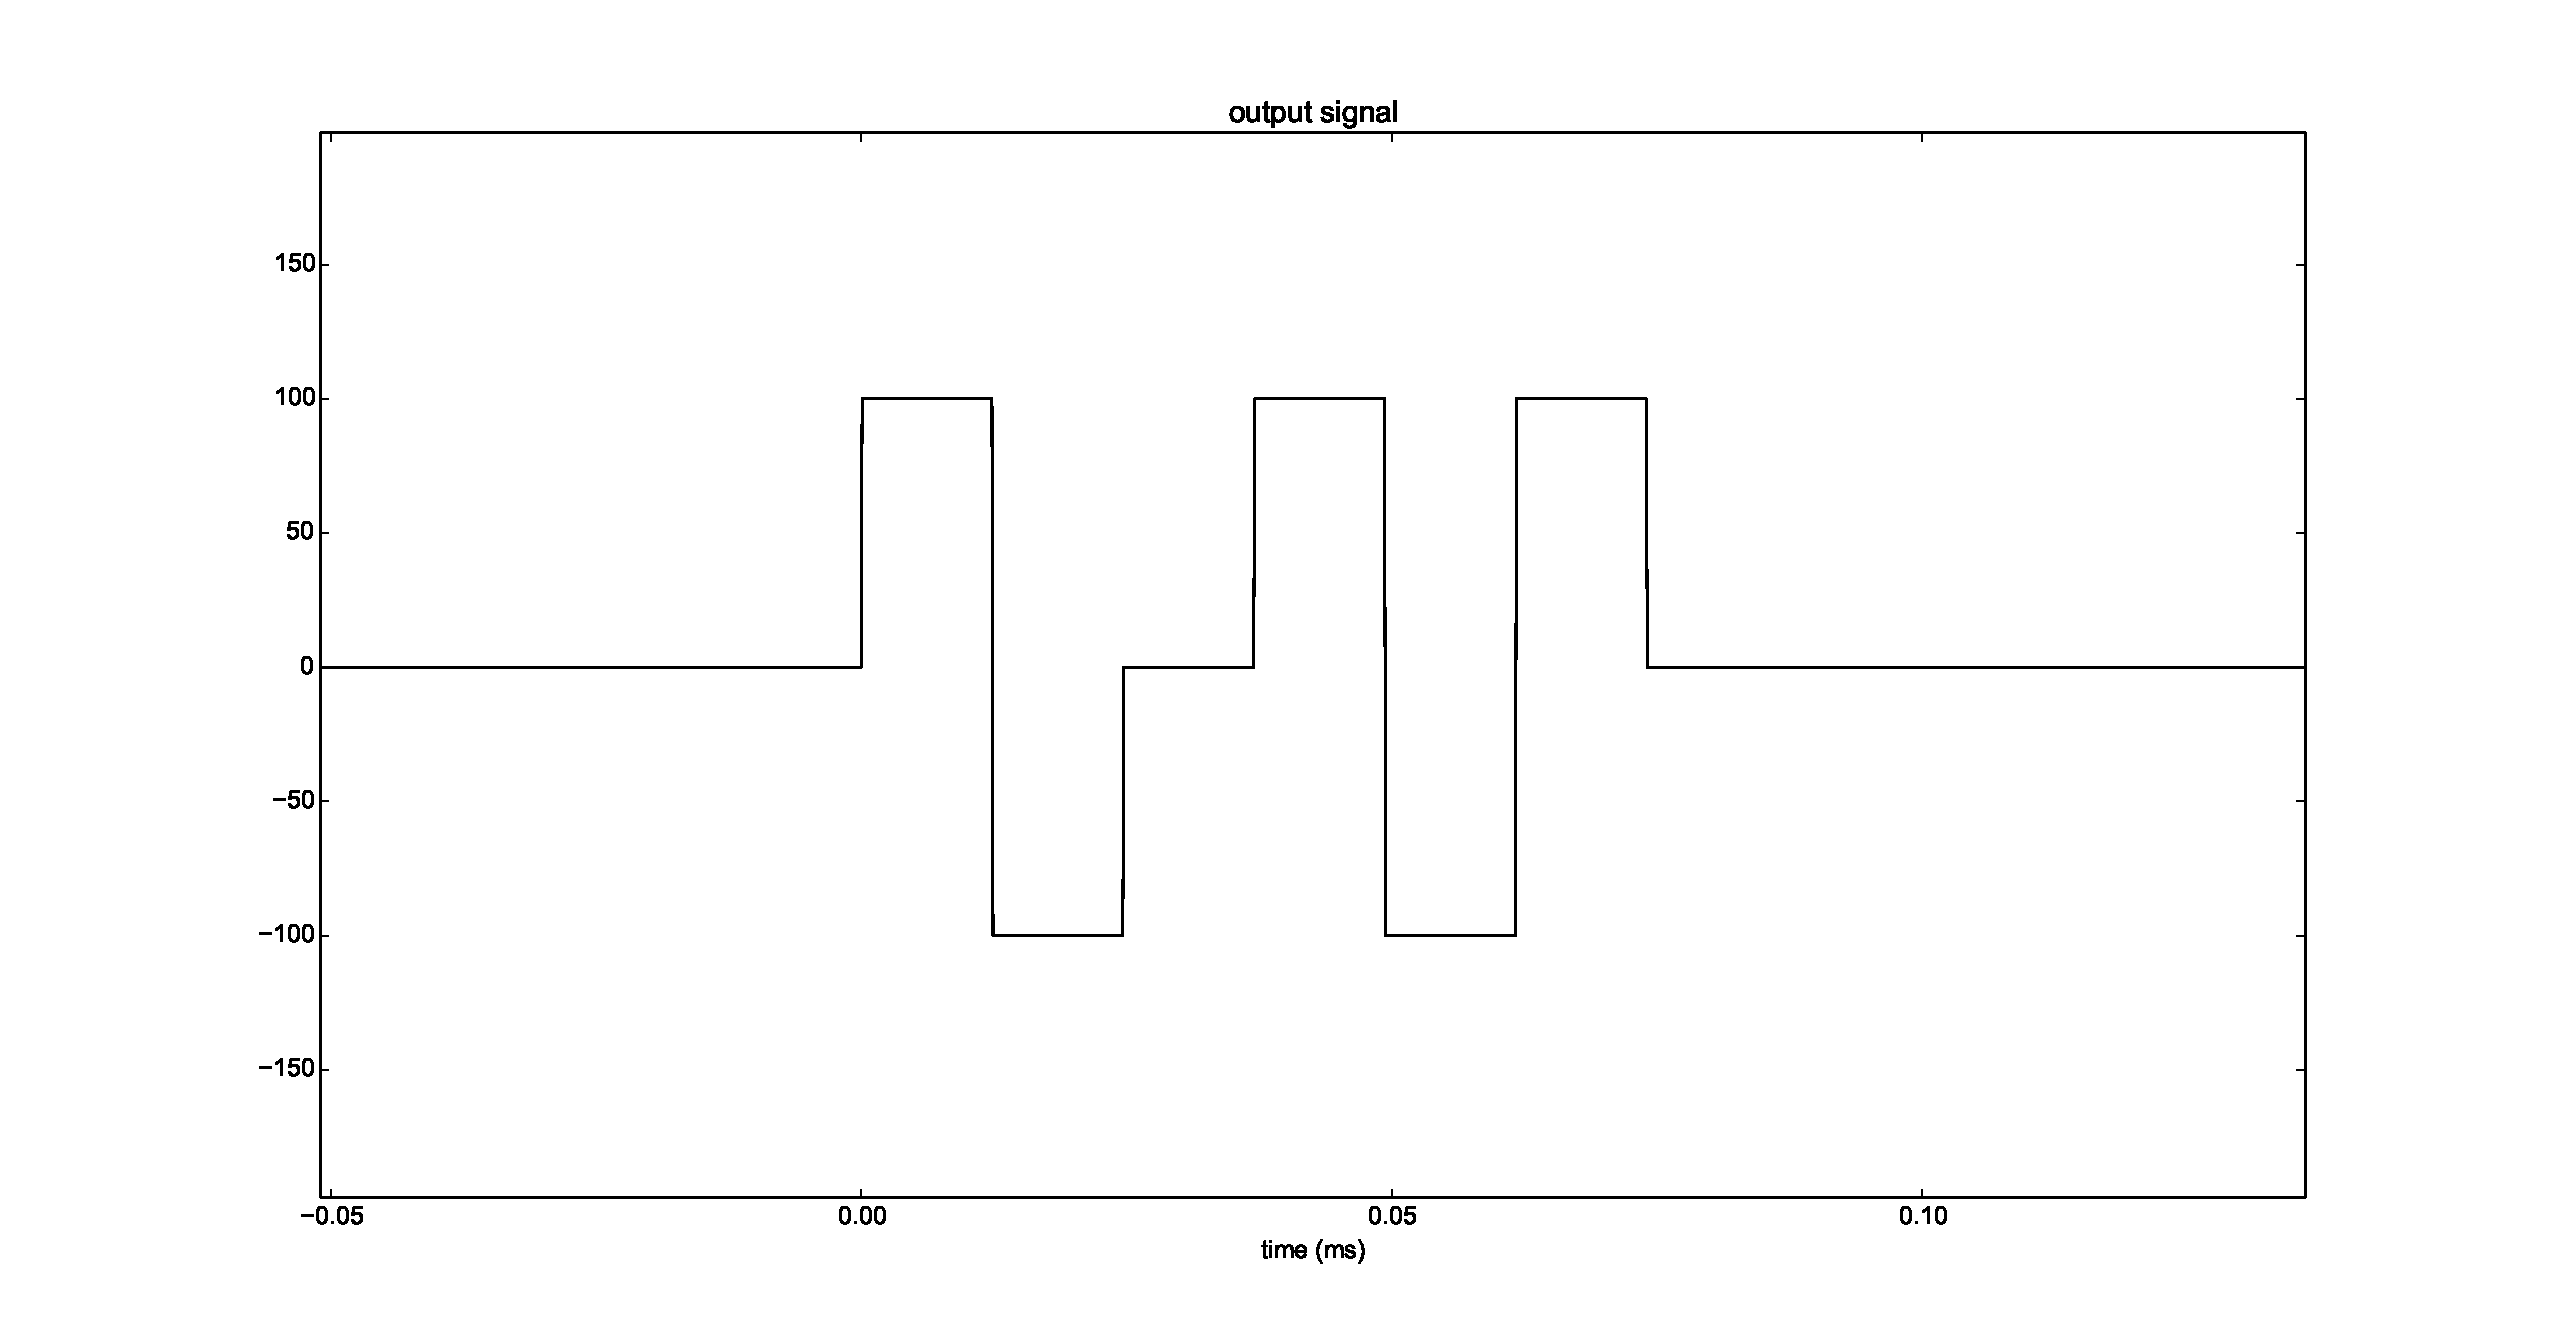
\includegraphics[width=1.15\textwidth, trim= 47mm 0mm 0mm 0mm,clip]{output_signal}
    \caption{sygnał wysterowania nadajnika piezoelektrycznego}
    \label{fig:output_signal}
\end{figure}


\section{Dobór rezonatorów piezoelektrycznych}
Głównym problemem podczas konstrukcji nadajnika okazał się dobór odpowiednich rezonatorów piezoelektrycznych.
Mimo, że producent zapewnia zakres pracy rezonatorów w zakresie: $40 kHz \pm 1kHz$, taki rozrzut okazał się niewystarczający, 
dlatego z 30 rezonatorów (15 nadajników i 15 odbiorników) wybrane zostały 4 nadajniki i 3 odbiorniki o najbardziej 
zbliżonych częstotliwościach pracy. Częstotliwość mierzona była za pomocą odpowiedzi rezonatora na 
krótki impuls elektryczny, sam pomiar dokonywany był na oscyloskopie cyfrowym. Poniżej wartości jakie udało się zmierzyć,
gwiazdką zaznaczone zostały wykorzystane rezonatory:

\begin{center}
  \begin{tabular}{|r|r|r|}
    \hline 
    nr & nadajnik: 40ST-12 & odbiornik: 40SR-12\\
    \hline
    1  &   40.88kHz & *40.65kHz \\
    2  &   41.12kHz &  40.45kHz \\
    3  &  *40.78kHz &  39.52kHz \\
    4  &   41.19kHz &  40.47kHz \\
    5  &   40.92kHz &  40.66kHz \\
    6  &   39.68kHz & *40.69kHz \\
    7  &   39.78kHz &  40.59kHz \\
    8  &  *40.80kHz &  40.39kHz \\
    9  &   40.90kHz &  40.29kHz \\
    10 &  *40.66kHz & *40.68kHz \\
    11 &  *40.85kHz &  39.22kHz \\
    12 &   41.01kHz &  39.51kHz \\
    13 &   41.00kHz &  39.92kHz \\
    
    14 &   39.82kHz &  39.26kHz \\
    15 &   39.64kHz &  39.11kHz \\
    \hline
  \end{tabular}
\end{center}


